% Inline licence here

\documentclass[a4paper,12pt]{report}

% Include Packages
\usepackage[a4paper,left=2.5cm,top=2.5cm,bottom=2.5cm,
	right=2.5cm]{geometry}
\usepackage{url}
\usepackage{fancyhdr}
\usepackage{etoolbox}
\usepackage{titlesec}
\usepackage{graphicx}
\graphicspath{ {images/} }

%=============Formating============%
% Customize chapter 

\titleformat{\chapter}[block]{\LARGE\bfseries}{Chapter \thechapter}
{0.5em} % sep
{} % before-code
[] % after-code
\titlespacing*{\chapter}{0pt}{-10pt}{40pt}

% Page Header and Footer
\pagestyle{fancy}
\rhead{\textbf{MiniSat}}
\chead{}
\lhead{}
\lfoot{Department of Computer Science and Engineering. RIT,Rajaramnagar}
\cfoot{}
\rfoot{\thepage}
\renewcommand{\footrulewidth}{.4pt}
\renewcommand{\headrulewidth}{.4pt}


% Redefine for plain styling page
\fancypagestyle{plain}{
\rhead{}
\chead{}
\lhead{}
\lfoot{Department of Computer Science and Engineering. RIT,Rajaramnagar}
\cfoot{}
\rfoot{\thepage}
\renewcommand{\headrulewidth}{0pt}
\renewcommand{\footrulewidth}{.4pt}
}


%% To check font size %%
\makeatletter
\newcommand{\showfontsize}{\f@size{} pt}
\makeatother

\begin{document}
\tableofcontents{}

\chapter{Introduction}
Cloud computing is the delivery of computing services-servers, storage, databases,
networking, software, analytics and more—over the Internet (“the cloud”). Companies
offering these computing services are called cloud providers and typically charge for cloud
computing services based on usage, similar to how you are billed for water or electricity at
home.\\
You are probably using cloud computing right now, even if you don’t realise it. If you use an
online service to send email, edit documents, watch movies or TV, listen to music, play
games or store pictures and other files, it is likely that cloud computing is making it all
possible behind the scenes. The first cloud computing services are barely a decade old, but
already a variety of organisations—from tiny startups to global corporations, government
agencies to non-profits—are embracing the technology for all sorts of reasons. Here are a
few​ ​ of​ ​ the​ ​ things​ ​ you​ ​ can​ ​ do​ ​ with​ ​ the​ ​ cloud:\\

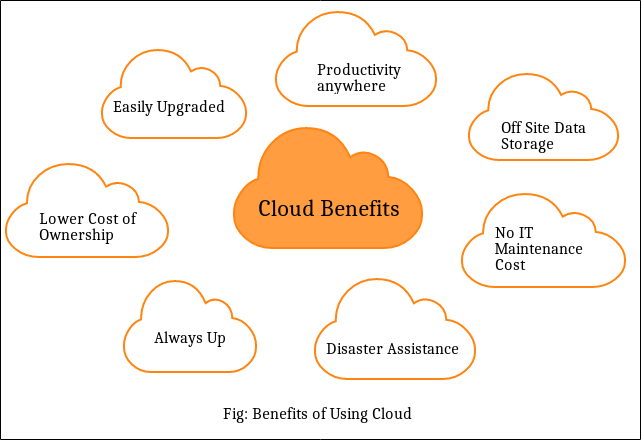
\includegraphics[scale=.65]{benefits_of_cloud}\\

\begin{itemize}
	\item Create​ ​ new​ ​ apps​ ​ and​ ​ services
	\item Store, back​ up​ ​ and​ ​ recover​ ​ data
	\item Host​ ​ websites​ ​ and​ ​ blogs
	\item Stream​ ​ audio​ ​ and​ ​ video
	\item Deliver​ ​ software​ ​ on​ ​ demand
	\item Analyse​ ​ data​ ​ for​ ​ patterns​ ​ and​ ​ make​ ​predictions\\
\end{itemize}
\textbf{Types​ ​ of​ ​ cloud​ ​ services:​ ​ IaaS,​ ​ PaaS,​ ​ SaaS}
Most cloud computing services fall into three broad categories: infrastructure as a service
(IaaS), platform as a service (PaaS) and software as a service (Saas). These are
sometimes called the cloud computing stack, because they build on top of one another.
Knowing what they are and how they are different makes it easier to accomplish your
business​ ​ goals.\\
\newline
\textbf{Infrastructure-as-a-service​ ​ (IaaS)}\\
The most basic category of cloud computing services. With IaaS, you rent IT
infrastructure—servers and virtual machines (VMs), storage, networks, operating
systems—from​ ​ a ​ ​ cloud​ ​ provider​ ​ on​ ​ a ​ ​ pay-as-you-go​ ​ basis.\\
The​ ​ benefits​ ​ of​ ​ IaaS
\begin{itemize}
	\item No​ ​ need​ ​ to​ ​ invest​ ​ in​ ​ your​ ​ own​ ​ hardware
	\item Infrastructure​ ​ scales​ ​ on​ ​ demand​ ​ to​ ​ support​ ​ dynamic​ ​ workloads
	\item Flexible,​ ​ innovative​ ​ services​ ​ available​ ​ on​ ​ demand\\
\end{itemize}
\textbf{Platform​ ​ as​ ​ a ​ ​ service​ ​ (PaaS)}\\
Platform-as-a-service (PaaS) refers to cloud computing services that supply an on-demand
environment for developing, testing, delivering and managing software applications. PaaS is
designed to make it easier for developers to quickly create web or mobile apps, without
worrying about setting up or managing the underlying infrastructure of servers, storage,
network​ ​ and​ ​ databases​ ​ needed​ ​ for​ ​ development\\.
The​ ​ benefits​ ​ of​ ​ PaaS
\begin{itemize}
	\item Develop​ ​ applications​ ​ and​ ​ get​ ​ to​ ​ market​ ​ faster
	\item Deploy​ ​ new​ ​ web​ ​ applications​ ​ to​ ​ the​ ​ cloud​ ​ in​ ​ minutes
	\item Reduce​ c ​ omplexity​ ​ with​ ​ middleware​ ​ as​ ​ a ​ ​ service\\
\end{itemize}
\textbf{Software​ ​ as​ ​ a ​ ​ service​ ​ (SaaS)}\\
Software-as-a-service (SaaS) is a method for delivering software applications over the
Internet, on demand and typically on a subscription basis. With SaaS, cloud providers host
and manage the software application and underlying infrastructure and handle any
maintenance, like software upgrades and security patching. Users connect to the
application​ ​ over​ ​ the​ ​ Internet,​ ​ usually​ ​ with​ ​ a ​ ​ web​ ​ browser​ ​ on​ ​ their​ ​ phone,​ ​ tablet​ ​ or​ ​ PC.\\
The​ ​ benefits​ ​ of​ ​ SaaS
\begin{itemize}
	\item You​ ​ can​ ​ sign​ ​ up​ ​ and​ ​ rapidly​ ​ start​ ​ using​ ​ innovative​ ​ business​ ​ apps
	\item Apps​ ​ and​ ​ data​ ​ are​ ​ accessible​ ​ from​ ​ any​ ​ connected​ ​ computer
	\item No​ ​ data​ ​ is​ ​ lost​ ​ if​ ​ your​ ​ computer​ ​ breaks,​ ​ as​ ​ data​ ​ is​ ​ in​ ​ the​ ​ cloud
	\item The​ ​ service​ ​ is​ ​ able​ ​ to​ ​ dynamically​ ​ scale​ ​ to​ ​ usage​ ​ needs\\
\end{itemize} 
\textbf{\large{Red​ ​ Hat​ ​ Satellite}} \\
\newline
\textbf{Provisioning}\\
Provision on bare metal, virtualized infrastructure, public or private
clouds—all​ ​ from​ ​ 1 ​ ​ centralized​ ​ console​ ​ and​ ​ with​ ​ 1 ​ ​ standardized​ ​ process.\\
\newline
\textbf{Configuration}\\
Configure your Red Hat systems in a more agile and efficient way. Analyze
and automatically remediate configuration drift and control, and enforce the
desired​ ​ host​ ​ end​ ​ state,​ ​ all​ ​ from​ ​ 1 ​ ​ convenient​ ​ console.\\
\newline
\textbf{Software​ ​ management}\\
Use a systematic process to apply content—including patches—to deployed
systems in all stages, from development to production. The result is better
consistency and availability of systems, letting IT more quickly respond to
business​ ​ needs​ ​ and​ ​ vulnerabilities.\\
\newline
\textbf{Subscription​ ​ management}\\
Report and map your Red Hat-purchased products to registered systems
for​ ​ end-to-end​ ​ visibility​ ​ into​ ​ subscription​ ​ usage​ ​ details.


\newpage
\chapter{Problem Statement}
"\textbf{MiniSat}​ ​ - ​ ​ A ​ ​ web​ ​ based​ ​ portal​ ​ to​ ​ provision​ ​ Vm.
Minisat​ ​ offers​ ​ a ​ ​ powerful​ ​ set​ ​ of​ ​ system​ ​ management​ ​ tools,​ ​ from​ ​ process​ ​ automation​ ​ to
security​ ​ compliance​ ​ and​ ​ more.​ ​ Here's​ ​ how​ ​ to​ ​ get​ ​ started."\\
\newline
As​ ​ your​ ​ organization​ ​ grows,​ ​ so​ ​ does​ ​ your​ ​ workload—and​ ​ the​ ​ IT​ ​ resources​ ​ required​ ​ to​ ​ manage​ ​ it.​ ​ There
is​ ​ no​ ​ "one-size-fits-all"​ ​ system​ ​ management​ ​ solution,​ ​ but​ ​ a ​ ​ centralized,​ ​ open​ ​ source​ ​ tool​ ​ such​ ​ as
miniSat​ ​ can​ ​ help​ ​ you​ ​ manage​ ​ your​ ​ company's​ ​ IT​ ​ assets​ ​ by​ ​ provisioning,​ ​ maintaining,​ ​ and​ ​ updating​ ​ hosts
throughout​ ​ the​ ​ complete​ ​ lifecycle.\\
\newline
MiniSat​ ​ becomes​ ​ even​ ​ more​ ​ powerful​ ​ when​ ​ integrated​ ​ with​ ​ other​ ​ open​ ​ source​ ​ projects​ ​ and​ ​ plugins,
and​ ​ I ​ ​ will​ ​ discuss​ ​ these​ ​ in​ ​ more​ ​ detail​ ​ below.​ ​ To​ ​ get​ ​ started,​ ​ however,​ ​ let's​ ​ consider​ ​ key​ ​ functions​ ​ of​ ​ an
effective​ ​ system​ ​ management​ ​ tool.\\
\newline
MiniSat​ ​ and​ ​ essential​ ​ system​ ​ management​ ​ areas
An​ ​ effective​ ​ systems​ ​ management​ ​ tool​ ​ should​ ​ address​ ​ all​ ​ of​ ​ these​ ​ key​ ​ areas.
Host​ ​ provisioning​ ​ is​ ​ for​ ​ deploying​ ​ instances​ ​ or​ ​ virtual​ ​ machines​ ​ on​ ​ bare-metal,​ ​ on-premises,​ ​ or​ ​ a ​ ​ cloud
provider's​ ​ data​ ​ center.\\
\newline
Content​ ​ management​ ​ refers​ ​ to​ ​ publishing,​ ​ promoting,​ ​ and​ ​ managing​ ​ various​ ​ versions​ ​ of​ ​ repositories
and​ ​ packages​ ​ in​ ​ the​ ​ CDN​ ​ and​ ​ systems​ ​ across​ ​ the​ ​ life​ ​ cycle​ ​ (i.e.,​ ​ development,​ ​ testing,​ ​ QA,​ ​ and
production).
Patch/errata​ ​ management​ ​ includes​ ​ bug​ ​ fixes​ ​ and​ ​ advisory​ ​ or​ ​ enhancement​ ​ packages.​ ​ An​ ​ effective
systems​ ​ management​ ​ tool​ ​ should​ ​ identify​ ​ applicable​ ​ errata​ ​ regularly​ ​ and​ ​ patch​ ​ registered​ ​ systems promptly.\\
\newline
Health​ ​ monitoring​ ​ and​ ​ reporting​ ​ enables​ ​ real-time​ ​ system​ ​ checkups.​ ​ This​ ​ should​ ​ include​ ​ updates,errata,​ ​ compliance,​ ​ workload,​ ​ and​ ​ system​ ​ performance​ ​ metrics​ ​ for​ ​ registered​ ​ hosts​ ​ and​ ​ running
services.
Remote​ ​ execution​ ​ is​ ​ for​ ​ running​ ​ arbitrary​ ​ commands​ ​ on​ ​ hosts​ ​ or​ ​ groups​ ​ of​ ​ hosts​ ​ to​ ​ perform​ ​ similar
activities​ ​ remotely.​ ​ These​ ​ commands​ ​ can​ ​ be​ ​ customized;​ ​ for​ ​ example,​ ​ to​ ​ provision​ ​ templates​ ​ or
partition​ ​ tables.\\
\newline
Identity​ ​ and​ ​ policy​ ​ lets​ ​ you​ ​ create​ ​ different​ ​ users​ ​ and​ ​ roles​ ​ and​ ​ manage​ ​ various​ ​ permission​ ​ policies.​ ​ This
function​ ​ should​ ​ also​ ​ support​ ​ Kerberos​ ​ and​ ​ LDAP​ ​ integration​ ​ and​ ​ authentication.
Alerts​ ​ and​ ​ notification​ ​ audits​ ​ administrator​ ​ and​ ​ user​ ​ activities.​ ​ This​ ​ tool​ ​ should​ ​ instantly​ ​ detect​ ​ what
changes​ ​ are​ ​ made​ ​ in​ ​ each​ ​ node,​ ​ when​ ​ they​ ​ are​ ​ made,​ ​ and​ ​ where​ ​ potential​ ​ risk​ ​ may​ ​ exist.
Automation​ ​ applies​ ​ to​ ​ repetitive​ ​ tasks.​ ​ A ​ ​ top​ ​ systems​ ​ management​ ​ tool​ ​ should​ ​ help​ ​ identify​ ​ and
automate​ ​ these​ ​ processes.

\chapter{Literature Survey}

Linux is a name which broadly denotes a family of free and open-source software operating system distributions built around the Linux kernel. The defining component of a Linux distribution is the Linux kernel, an operating system kernel first released on September 17, 1991 by Linus Torvalds.\\
\newline
Typically, Linux is packaged in a form known as a Linux distribution for both desktop and server use. Some of the most popular and mainstream Linux distributions are Arch Linux, CentOS, Debian, Fedora, Gentoo Linux, Linux Mint, Mageia, openSUSE and Ubuntu, together with commercial distributions such as Red Hat Enterprise Linux and SUSE Linux Enterprise Server.\\
\newline
In many ways, Linux is similar to other operating systems you may have used before, such as Windows, OS X, or iOS. But Linux also is different from other operating systems in many important ways. First, and perhaps most importantly, Linux is open source software. The code used to create Linux is free and available to the public to view, edit, and—for users with the appropriate skills—to contribute to.\\
\newline
Linux is also different in that, although the core pieces of the Linux operating system are generally common, there are many distributions of Linux, which include different software options. This means that Linux is incredibly customizable, because not just applications, such as word processors and web browsers, can be swapped out.\\
\newline
Git is a free and open source distributed version control system designed to handle everything from small to very large projects with speed and efficiency. Git was created by Linus Torvalds in 2005 for development of the Linux kernel, with other kernel developers contributing to its initial development. 2.15 is the latest git version released on 2017-10-30.\\
\newline
Virtualization is technology that allows you to create multiple simulated environments or dedicated resources from a single, physical hardware system. Software called a hypervisor connects directly to that hardware and allows you to split 1 system into separate, distinct, and secure environments known as virtual machines (VMs). These VMs rely on the hypervisor’s ability to separate the machine’s resources from the hardware and distribute them appropriately.\\

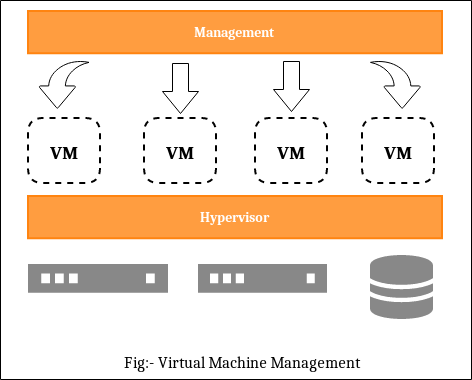
\includegraphics[scale=.85]{vm_management}\\

Types of virtualization:
\begin{itemize}
	\item Server Virtualization
	\item OS Virtualization
	\item Network Virtualization
	\item Hardware Virtualization
	\item Application Virtualization
	\item Storage Virtualization\\
\end{itemize}
Django is a free and open source web application framework, written in Python. A web framework is a set of components that helps you to develop websites faster and easier.
When you're building a website, you always need a similar set of components: a way to handle user authentication (signing up, signing in, signing out), a management panel for your website, forms, a way to upload files, etc. \\
\newline
Other people long ago noticed that web developers face similar problems when building a new site, so they teamed up and created frameworks (Django being one of them) that give you ready-made components to use.
Frameworks exist to save you from having to reinvent the wheel and to help alleviate some of the overhead when you’re building a new site. \\
\newline
To understand what Django is actually for, we need to take a closer look at the servers. The first thing is that the server needs to know that you want it to serve you a web page.\\
\newline
Imagine a mailbox (port) which is monitored for incoming letters (requests). This is done by a web server. The web server reads the letter and then sends a response with a webpage. But when you want to send something, you need to have some content. And Django is something that helps you create the content.



\chapter{National/International Status}

Since 2000, cloud computing has come into existence. In early 2008, NASA's OpenNebula, enhanced in the RESERVOIR European Commission-funded project, became the first open-source software for deploying private and hybrid clouds, and for the federation of clouds. In the same year, efforts were focused on providing quality of service guarantees (as required by real-time interactive applications) to cloud-based infrastructures, in the framework of IRMOS European Commission-funded project, resulting in a real-time cloud environment.\\

In August 2006 Amazon introduced its Elastic Compute Cloud. Microsoft Azure was announced as "Azure" in October 2008 and was released on 1 February 2010 as Windows Azure, before being renamed to Microsoft Azure on 25 March 2014.\\

In July 2010, Rackspace Hosting and NASA jointly launched an open-source cloud-software initiative known as OpenStack. The OpenStack project intended to help organisations offering cloud-computing services running on standard hardware. The early code came from NASA's Nebula platform as well as from Rackspace's Cloud Files platform. As an open source offering and along with other open-source solutions such as CloudStack, Ganeti and OpenNebula, it has attracted attention by several key communities. Several studies aim at comparing these open sources offerings based on a set of criteria.\\
In computing, Red Hat Satellite[2] is a systems-management product by the company Red Hat which allows system administrators to deploy and manage Red Hat Enterprise Linux (RHEL) hosts.

A Satellite server registers with Red Hat Subscription Management, mirrors all relevant software like security errata and bug fixes, and provides this together with locally added software and configuration to the attached servers.

The managed hosts register against the local Satellite server and access the provided resources like software packages, patches, configuration, etc. while they also provide information about the current health state of the server to the Satellite. \\
Component on Red Hat Satellite
\begin{itemize}
	\item The Foreman
	\item Katello
	\item Candlepin
	\item Pulp
	\item Hammer
	\item REST API
	\item Apache Tomcat
	\item Puppet
	\item Hiera
\end{itemize}

\chapter{Applications}
Virtualization isn't just for geeks or those who run enormously powerful servers. It offers something for everybody, and if you haven't yet dipped your toe into the virtualization ocean, then you're at serious risk of being left behind.\\
\newline
In its strictest sense, virtualization refers to running two or more operating systems one one physical PC. Either the multiple operating systems run side-by-side, with a separate piece of software called a hypervisor used to manage them, or one operating system runs the other operating systems within program windows. The former is usually limited to servers, with the latter finding common use on desktop computers.
Here are various things you can do with virtualization that might convince you that it's worth giving it a try, if you haven't already.\\
\newline
\textbf{Run Old Apps}\\
Got an application that won't play nice in Windows 7 or Vista, but works fine in XP or an even earlier version of Windows, like Me? Just grab an old Windows CD and install it within a virtual machine (VM). Then install your app.\\
\newline
VMware Player features Unity mode, which allows applications running in the virtual machine to appear as if they're running natively on the host computer. They have their own taskbar buttons and their own program windows, making for a seamless experience. For this to work, however, you'll need to install the VMware Tools program on the virtualized operating system. You're usually prompted to do this after installation of the OS has finished.\\
\newline
\textbf{Browse in Complete Safely}\\
Why not install Windows on VMware Player, then install Firefox, and run it in Unity mode so it appears to run natively on the host computer?
Essentially Firefox will be running in what's known as a sandbox, meaning that should it (or one of its plugins) get hacked while you're online, there'll be no absolutely no risk to your actual operating system. You could create a snapshot once everything's been configured in the virtual machine in order to get things back up and running quickly, should anything go wrong.\\
\newline
\textbf{ Back Up an Entire Operating System}\\
Because the virtual OS is entirely contained within a series of files, backing it up is as simple as backing up any other files. It's the same with virtualized server installations too. If you're running a virtual machine on a server to host your mail server, and it's brought down by a hack attack, then bringing things back to working order is as simple as restoring the backup files (assuming the vulnerability that allowed the hack is quickly addressed once things are up and running, of course).
Bear in mind that creating a copy of a VM creates legal issues. Backing up should be fine, but if you create a copy of a VM installation to give to a friend, for example, then you'll be contravening copyright laws (assuming they apply, as with Microsoft, but not always with Linux).\\
\newline
\textbf{ Create a Personal Cloud Computer}\\
If you're out of the office, there's no need to take your laptop with you. Just leave it running (with power saving turned off!), take your mobile phone or tablet computer instead, and access the laptop via a Remote Desktop Protocol (RDP) connection over the Internet. This will let you access the same desktop environment you're used to, although there'll be no fancy graphics.\\
\newline
You'll need to take a note of the public IP address of your router in order to connect remotely, and configure the router to port forward incoming RDP connections to your notebook PC. How this is done varies from computer to computer, but often you can select predefined rules.
Then download an RDP client for your mobile device and connect. For the Apple iPad and iPhone, you can try iTap but there are DP clients for most platforms.\\
\newline
\textbf{Reuse Old Hardware}\\
By installing Citrix XenDesktop on your Windows server, you can turn old, less powerful computers into thin clients, wiping out the need for a workstation IT upgrade budget.\\
\newline
The clients access their personal desktop spaces on the server and there's little noticeable difference compared with running the operating system and applications locally. XenDesktop includes clever technology to avoid common thin-client pitfalls, such as the fact videos and animations don't play well, by shifting some of the processing work to the client computer.
XenDesktop also allows your workers to access their desktops from home, provided the server is configured to be publicly accessible and they have the right client software installed. You can even use mobile phones to connect to the desktop environments.




\chapter{Objectives of Project}
\begin{enumerate}
	\item User should​ ​ be​ ​ able​ ​ to​ ​ login​ ​ application​ ​ with​ ​ ldap​ ​ authentication​ ​ on​ ​ application.
	\item User should be able to provision host with different provider such as libvirt,	docker​ ​ container​ ​ etc.
	\item User should be able to configure network and storage, select type of provider,
	type​ ​ of​ ​ operating​ ​ system​ ​ and​ ​ contents.
	\item User should be able to register already provisioned host within network to
	application.(Existing machine having already installed operating system can
	fetch​ ​ packages​ ​ from​ ​ server​ ​ application)
	\item User should be able to register already provisioned host within network to
	application.(Existing machine having already installed operating system can
	fetch​ ​ packages​ ​ from​ ​ server​ ​ application)
	\item User should​ ​ be​ ​ able​ ​ to​ ​ sync​ ​ content​ ​ from​ ​ application​ ​ to​ ​ host.
	\item User should​ ​ be​ ​ able​ ​ to​ ​ get​ ​ system​ ​ health
	
\end{enumerate}

\chapter{Future Scope}
Adoption of cloud computing technology has significantly increased over the last few years, promising a great opportunity for innovation amongst businesses. However some businesses are still sceptical of how Cloud Computing can enhance or replace all or part of their IT environment.\\
\newline
Cloud is typically marketed to promote benefits such as improved efficiency, flexibility and even opportunity for expansion. However many of these benefits lack tangibility, often making it difficult to validate a move to the cloud.\\
\newline
Organisations considering the change typically look at implementing a solution that incorporates a mix of on premise, and public or private cloud, referred to as a hybrid cloud model.\\
\newline
Business continuity has been identified as one of the most important elements of business operations. A business continuity solution is not just simply backing up and/or replicating content to the cloud, nor is it simply a Disaster Recovery plan. Business continuity is to continue to do business during a failure or disaster. In basic terms, it means that when a failure or disaster happens, that data is still accessible with little to no downtime.\\
\newline
A business continuity solution therefore needs to be planned to consider key elements such as resilience, recovery and contingency. Hybrid cloud solutions are often considered by organisations as a key component of a business continuity solution where critical data is replicated to a cloud solution in a different location to the primary systems. This provides data insurance in the event of a disaster (natural or technological), minimising downtime and the costs associated with such an event. Understanding this benefit, service providers have streamlined their offerings to easily integrate a business continuity solution into hybrid cloud systems.\\
\newline
Barriers to innovation are reduced in a cloud environment, as large capital expenditure is not required for modelling a new service. Previously, cost associated with such a task would include capital expenditure for infrastructure, labour and time for research then more resources to install and maintain. This places a lot of pressure on capacity management practices and perfect forecasting despite many uncertain variables. In hybrid cloud, concepts can be tested without capital expenditure, prototyped in a cloud environment then rapidly deployed and measured for success. The added benefit of hybrid cloud is the availability of resources combining both internal and external environments including data, network, and infrastructure, all available on iseek’s cloud environment.\\
\newline
Scaling on IT infrastructure can be extremely expensive, inefficient and places much more pressure on accurate forecasting in growing companies. However, a hybrid cloud environment can provide the opportunity for businesses to scale out to a cloud environment for specific workloads. Implementing automation rules on the cloud provides the ability to scale resources up and down as business demands change. This allows the hybrid cloud system to take advantage of unlimited resources based on demand driven usage, optimising the environment for performance and efficiency.\\
\newline
In many organisations, speed to market is a key differentiator. In a digital age, the ability to quickly spin up environments to test, prototype and launch new products is highly desirable. For organisations with an IT infrastructure that is working near or close to capacity, spinning up a new environments can become a challenge and potentially hinder the business\\
\newline
Hybrid cloud allows resources to be deployed and commissioned in an automated process that can yield results at hugely improved speeds, so companies are no longer limited by their IT footprint.\\
\newline
Companies can leverage hybrid cloud as the first step in moving to a predominately cloud environment. A hybrid solution provides the perfect opportunity for companies to test the capability of certain workloads and providers in a cloud based environment and assist them in planning their cloud strategy. However planning is key, as hybrid cloud can require complex design to coherently combine an organisation’s platform with a cloud environment.

\chapter{Methodology}

Began with learning the term "Virtualization". Virtualization is technology
that allows you to create multiple simulated environments or dedicated resources
from a single, physical hardware system. Software called a hypervisor connects
directly to that hardware and allows you to split 1 system into separate, distinct,
and secure environments known as virtual machines (VMs). These VMs rely on
the hypervisor’s ability to separate the machine’s resources from the hardware and
distribute​ ​ them​ ​ appropriately.\\
\newline
To create VM on linux operating system we have tools like virt-manager
which uses Libvirt APIs. Started with creating VM on same machine and then
moved further and tried creating VM on another machine in same network.
Developed a script to automatically deploy VM on the target machine by taking
input from client. Designed a GUI using Django to provide easy to user in
generating​ ​ VM​ ​ of​ ​ its​ ​ own​ ​ desire.\\
\newline
\textbf{Setup project environment}\\
Two machine with 16GB RAM and four CPUs. The system is installed using Fedora 26 operating system. Fedora 26 is a linux flavour with linux kernel. The should have libvirt and lxc installed in there system. \\
\newline
\textbf{Creating a local repository}
To provision a virtual machine we need a operating system. We cant download operating system every time we provision a virtual machine So we create a mirror of different operating system. We use rsync a cli tool to mirror a repository. \\
\newline
\textbf{Creating a python package}\\
We are planning on creating a python package which will work as API. We will use the API function to provision virtual machine and run docker container. \\
\newline
\textbf{Developing a WebUI}\\
Using django we will create a centrilize a WebUI which will be used to provision virtual machine and run docker container. We will import the python package. \\
\newline
\textbf{Create documentation}\\
Doing a task is must, but its documentation is more valuable as that of project. The details of the projects are to be documented with all the installation procedure and the actual flow of project implementation to help other people understand the project brightly.\\

\chapter{Conclusion}
With MiniSat we will  be a able to simplify day to day task for system administrator.\\
The task will include: \\
\newline
\textbf{Provision}
Satellite offers numerous methods for deploying hosts, including simple kickstart, bare metal install and re-imaging. Current versions of Satellite support kickstart using Cobbler as an underlying framework. PXE Boot, and Koan are methods that can be used to implement bare metal installs and re-imaging of hosts. \\
\newline
\textbf{Manage}
Satellite assists in remotely managing hosts in several areas: software, operational management, and configuration. The main mechanisms for managing hosts are:
\begin{itemize}
	\item Software Channels
	\item Configuration Channels
	\item Activation Keys\\
\end{itemize}
\textbf{Monitor}
Satellite can provide monitoring of software and systems via probes. These probes periodically explore the target host and send alerts if the probes do not get the correct replies, or if the replies fall outside of upto specified range.\\
\newline
For a system administrator this task are very important and if there are hundreds on different machine which require monitoring, for system monitor it is like a nightmare. So I hope MiniSat will help administrator and simplify there task.

\chapter{References}
\begin{enumerate}
	\item Project Link\\
	\newline
	https://github.com/miniSat
	
	\item Documentation\\
	\newline
	https://github.com/rh-universityoutreach-india/projects/pull/20\\
	https://access.redhat.com/documentation/en/red-hat-satellite/6.2/paged/architecture-guide/12-system-components\\
	https://en.wikipedia.org/wiki/Cloud-computing\\
	https://en.wikipedia.org/wiki/Virtualization\\
	
\end{enumerate}
\end{document}

